%\documentclass{article}

%%%%
% PLOTS mapas
% eval=FALSE
% results=HIDE (verbatim default)
%%%%
%\usepackage[utf8]{inputenc}
%\usepackage{longtable}
%\usepackage{authblk}
%\usepackage{adjustbox}

%%%%
%\begin{document}
\Sconcordance{concordance:basico32departamentos.tex:basico32departamentos.Rnw:%
1 18 1 1 9 2 1 1 31 6 1 1 12 1 4 1 1 1 12 1 5 1 1 1 27 4 1 1 27 1 2 16 %
1}

%\SweaveOpts{concordance=TRUE}
%\SweaveOpts{concordance=TRUE}

%Partes extras para las nuevas columnas
% Exploracion Univariada --------------------------------------------------

\section{Exploración Espacial}

El siguiente mapa muestra el impacto que tiene la población de cada departamento sobre su respectivo IDH:





%con esto hagamos el merge:



 
 
\begin{figure}[h]
\centering
\begin{adjustbox}{width=8cm,height=6cm,clip,trim=1.5cm 2cm 0cm 2.5cm}
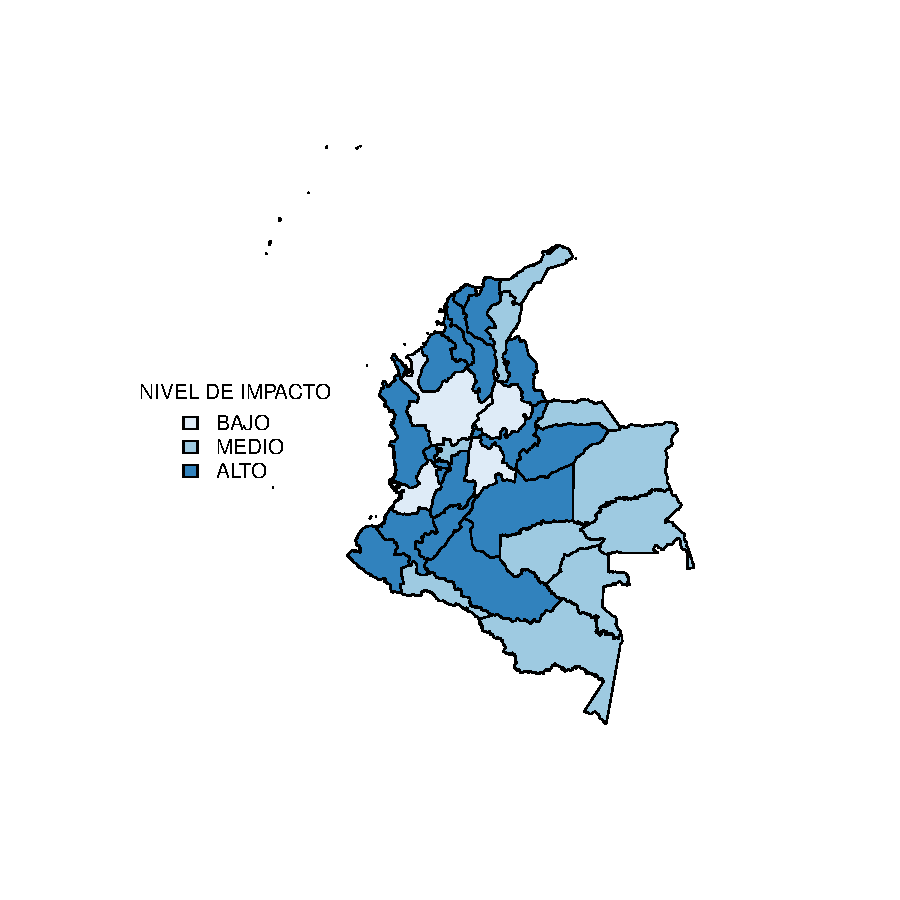
\includegraphics{basico32departamentos-plotMap0}
\end{adjustbox}
\caption{Impacto de población en IDH por departamento}\label{rawmap}
\end{figure}

Entre mayor es el impacto de la población sobre el IDH del departamento, más oscuro se muestra en el mapa. Se dividió el impacto en 3 niveles: BAJO, MEDIO Y ALTO.
Para lograr esta escala se implementó el siguiente procedimiento:

Primero se obtuvieron los datos de IDH, población de cabecera, el resto de la población y el total de la población de cada departamento del país.

Se limpiaron los datos reemplazando caracteres no reconocibles tales como la letra "ñ" y tildes.
Para evitar un sesgo significativo por variaciones amplias en número de habitantes, primero se utilizaron valores logarítmicos y luego se normalizaron. Finalmente se crearon las 3 agrupaciones por medio de la técnica K-means.


\endinput


%\end{document}
